\documentclass{article}

\usepackage{url}
\usepackage[hmargin=1.5in]{geometry}
\usepackage{enumitem}
\usepackage{amsmath}
\usepackage{amssymb}
\usepackage{amsthm}
\usepackage{eqnarray}
\usepackage{graphicx}
\usepackage[svgnames]{xcolor} %% for revisions
\usepackage{xparse} %% for squiggly underlines
\usepackage{tikz-cd} %% for term norm scratch work
\usepackage{tikz}

% TikZ libraries
\usetikzlibrary{bbox}
\usetikzlibrary{fadings}

% hat tip TeX.SE user Andrew Stacey
%   https://tex.stackexchange.com/a/82503/6934
%   https://tex.stackexchange.com/questions/82425/tikz-radial-shading-of-a-ring#comment176908_82503
\pgfdeclareradialshading{radialedge}{\pgfpointorigin}{%
  color(0bp)=(transparent!0);
  color(20bp)=(transparent!0);
  color(22bp)=(transparent!10);
  color(24bp)=(transparent!90);
  color(25bp)=(transparent!100)
}
\pgfdeclarefading{radial edge}{\pgfuseshading{radialedge}}%

%%\theoremstyle{definition}
\newtheorem{defn}{Definition}
\theoremstyle{plain}
\newtheorem{prop}{Proposition}
\newtheorem{lem}{Lemma}
\newtheorem{thm}{Theorem}
\newtheorem{rmk}{Remark}
\newtheorem{lemma}{Lemma}

% list formatting
\setlist[itemize]{leftmargin=24mm, rightmargin=12mm}
\makeatletter
% hat tip TeX.SE user31729
%   https://tex.stackexchange.com/a/328393/6934
\newcommand{\cond}[1]{\item[(\textsc{#1})]\protected@edef\@currentlabel{\textsc{#1}}}
\newcommand{\condconst}[2]{\item[($\text{\textsc{#1}} \mid #2$)]\protected@edef\@currentlabel{$\text{\textsc{#1}} \mid #2$}}
\makeatother

% convenience aliases
\newcommand{\maps}{\colon}

% group action
\newcommand{\acts}{\mathbin{\raisebox{\depth}{\rotatebox{-90}{$\circlearrowright$}}}}

% symbology
\newcommand{\Z}{\mathbb{Z}}
\newcommand{\R}{\mathbb{R}}
\newcommand{\C}{\mathbb{C}}
\let\Re\relax
\DeclareMathOperator{\Re}{Re}
\newcommand{\laplace}{\mathcal{L}}
\newcommand{\series}[1]{\tilde{#1}}
\newcommand{\fracderiv}[3]{\partial^{#1}_{#2, #3}}

% function spaces
\newcommand{\cont}{\mathcal{C}}
\newcommand{\holo}{\mathcal{H}}
\newcommand{\singexp}[2]{\mathcal{H}L^\infty_{#1, #2}}
\newcommand{\holoL}[1]{\mathcal{H}L^{#1}} %% may no longer be needed
\newcommand{\expHoloL}[2]{\mathcal{H}L^{#1}_{#2}} %% may no longer be needed

% operator under consideration
\newcommand{\volterra}{\mathcal{V}}
\newcommand{\hardpart}{\mathcal{V}_\text{basic}}
\newcommand{\softpart}{\mathcal{V}_\text{extra}}
\newcommand{\hardker}{k_\text{basic}}
\newcommand{\softker}{k_\text{extra}}

% domain
\newcommand{\domain}{\Omega}
\newcommand{\near}{\Omega_\text{near}}
\newcommand{\far}{\Omega_\text{far}}

% drafting environments
\newenvironment{verify}{\color{ForestGreen}}{\color{black}}

\title{Regular singular Volterra equations on complex domains}
\author{Aaron Fenyes and Veronica Fantini}
\date{}

\begin{document}
\maketitle
\section{Introduction}
\subsection{Motivation}\label{motivation}
In its most basic form, the Laplace transform $\laplace$ turns $L^1$ functions of a real ``position'' variable $\zeta$ into holomorphic functions of a complex ``frequency'' variable $z$. Through identities like
\begin{align*}
\frac{\partial}{\partial z} \laplace \varphi & = \laplace(z\varphi) \\
\laplace k\;\laplace \varphi & = \laplace(k * \varphi) \\
z^{-\lambda} \laplace \varphi & = \laplace\,\fracderiv{-\lambda}{}{} \varphi,
\end{align*}
where $\fracderiv{-\lambda}{}{}$ is the Riemann-Liouville fractional integral of order $\lambda \in (0, \infty)$, the Laplace transform pulls differential operators on the frequency domain back to Volterra integral operators on the position domain. The favorable regularity properties and comprehensive theory of Volterra equations can thus be brought to bear on differential equations.

If we complexify the position variable $\zeta$, the functions on the position domain whose Laplace transforms satisfy a given differential equation will often extend holomorphically. \textbf{[...]}
\subsection{Setting}\label{setting}
\subsubsection{The domain}\label{setting:domain}
Throughout this paper, as described in Section~\ref{motivation}, the ``position'' variable $\zeta$ will be the standard coordinate on $\C$. Take a simply connected open set $\domain \subset \C$ that touches but doesn't contain $\zeta = 0$. For some of our results, we'll need an extra condition on $\domain$:
\begin{itemize}
\cond{star}\label{cond:star} The set $\domain$ is star-shaped around $\zeta = 0$. In other words, for any $a \in \domain$, a straight path from $\zeta = 0$ to $a$ stays in $\domain$. Since $\domain$ doesn't contain $\zeta = 0$, we'll always leave that starting point out of the path.
\end{itemize}
For the applications we have in mind, $\domain$ might look something like the set pictured below, which satisfies Condition~\eqref{cond:star}.
\begin{center}
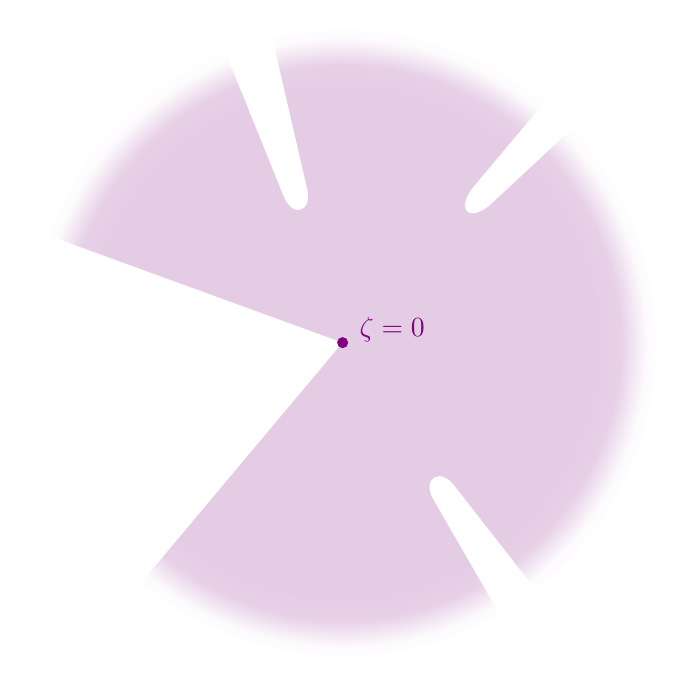
\begin{tikzpicture}
\newcommand{\spill}{4}
\fill[violet!20, bezier bounding box, path fading=radial edge]
  (-\spill, -\spill) (\spill, \spill)
  (0, 0) -- (160:\spill)
  arc (160:112:\spill) -- (112:2) .. controls (112:1.7) and (103:1.7) .. (103:2) -- (103:\spill)
  arc (103:50:\spill) -- (50:2.6) .. controls (50:2.2) and (43:2.2) .. (43:2.6) -- (43:\spill)
  arc (43:-52:\spill) -- (-52:2.3) .. controls (-52:2) and (-60:2) .. (-60:2.3) -- (-60:\spill)
  arc (-60:-130:\spill) -- (0, 0);
\fill[violet] circle (0.7mm) node[anchor=195, outer sep=1mm] {$\zeta = 0$};
\end{tikzpicture}
\end{center}
\subsubsection{The prototype operator}\label{setting:basic}
The prototypical example of the kind of operator we'll be working with is a holomorphic Volterra operator $\hardpart$ with a separable kernel and a regular singularity at $\zeta = 0$.

Being a holomorphic Volterra operator means that $\hardpart$ sends each holomorphic function $\varphi$ on $\domain$ to a new holomorphic function
\[ [\hardpart\,\varphi](a) = \int_{\zeta = 0}^a \hardker(a, \cdot)\,\varphi\;d\zeta. \]
Being separable means that the kernel $\hardker(a, a')$ factors into a function of $a$ times a function of $a'$. We'll suppose this product can be written as a ratio
\[ \hardker(a, a') = \textcolor{magenta}{-} \frac{q(a')}{p(a)}, \]
where $p$ and $q$ are holomorphic functions on $\domain$. Having a regular singularity at $\zeta = 0$ means that for some constant $\tau$---the {\em residue} of the singularity---the difference
\[ \hardker(a, a') \textcolor{magenta}{-} \frac{\tau}{\zeta(a)} \]
is bounded on a neighborhood of $\big(\zeta(a), \zeta(a')\big) = (0, 0)$ in $\Omega^2$. We'll assume that $\tau$ is real and positive.

Our definition of a regular singularity implies that as $|\zeta|$ goes to zero, $|p|$ also goes to zero, while $|q|$ settles into a compact interval that doesn't include zero.
\begin{verify}
[\textit{Proof.} Fix any $a'$ in the neighborhood where the difference above is bounded. By confining $a$ to small enough neighborhoods of $\zeta = 0$, we can make $|\tau/\zeta(a)|$ arbitrarily large, forcing $|q(a')/p(a)|$ to become arbitrarily large to satisfy the definition. Since $a'$ is fixed, the only way for this ratio to get arbitrarily large is for $|p(a)|$ to get arbitrarily small.]
\end{verify}
For some of our results, we'll also need to keep $|p|$ and $|q|$ under control as $|\zeta|$ goes to infinity.
\begin{itemize}
%%\item[($\text{\textsc{slow}} \mid \lambda_0$)]
\condconst{slow}{\lambda_0}\label{cond:slow} We can find constants $\lambda_p$ and $\lambda_\text{ratio}$ with
\begin{align*}
\left|\frac{1}{p}\right| & \lesssim e^{\lambda_p |\zeta|} &
\left|\frac{q}{p}\right| & \le \lambda_\text{ratio}
\end{align*}
outside some neighborhood of $\zeta = 0$ in $\Omega$. Note that this only constrains the ratio of $p$ and $q$ when they're evaluated at the same point. The constants will only enter our reasoning through their sum, $\lambda_0 = \lambda_p + \lambda_\text{ratio}$.
\end{itemize}
This condition explains why $\domain$ might have the sort of shape illustrated in Section~\ref{setting:domain}. As $\domain$ stretches out toward infinity, it has to part around the zeros of $p$, keeping well away from every zero except the one at $\zeta = 0$.
\subsubsection{The perturbed operator}\label{setting:perturbed}
\color{RoyalBlue}
We'll generalize $\hardpart$ by adding a perturbation $\softpart$ that doesn't have a separable kernel, but does have a smoothing effect that counteracts the singularity of $\hardpart$. To get the smoothing effect, we'll require the kernel $\softker$ of $\softpart$ to vanish to some order $\epsilon > 0$ on the diagonal in $\Omega^2$. This requirement, combined with two others, will be made precise in Condition~\eqref{cond:eps-lambda}.

Since $\softpart$ is a holomorphic Volterra operator, $\softker$ is a holomorphic function on $\domain^2$. We'll allow $\softker(a, a')$ to have a simple pole at $\zeta(a) = 0$, like $p(a)^{-1}$ does, but we won't allow any sharper singularity. We'll also put an exponential bound on how fast $\softker$ grows away from the diagonal, mimicking Condition~\eqref{cond:slow} on $p$ and $q$. Altogether, we'll require:
\begin{itemize}
\condconst{diag}{\epsilon, \lambda}\label{cond:eps-lambda} We have
\[ \big| k_\text{extra} (a, a') \big| \lesssim \textcolor{magenta}{C_k}\frac{|\zeta(a)-\zeta(a')|^\epsilon}{|\zeta(a)|}\,e^{\lambda|\zeta(a)-\zeta(a')|}\]
over all $a, a' \in \domain$.
\end{itemize}
\color{black}

Our ultimate goal is the study of certain integral equations where the integral kernel is a perturbation of $k_\text{basic}$. In particular, we are interested in holomorphic Volterra operators $\volterra=\hardpart+\softpart$, hence the kernel $k_\text{extra}$ of $\softpart$ is a holomorphic function on $\Omega^2$.  

For some of our results, we need to keep $k_\text{ext}$ under control at two different regimes: close to the point $\zeta=0$ and far toward infinity. In the former case, we require $k_\text{extra}$ to grow as $|\zeta|^{\epsilon-1}$ for some positive constant $\epsilon$; in the latter, we require $k_\text{ext}$ to be exponentially bounded
\begin{itemize}
\condconst{bounds}{\epsilon, \lambda}%%\label{cond:eps-lambda} (remove line break)
for every $a,a'\in\Omega$
\[ \big| k_\text{extra} (a, a') \big|\le C_{k}\frac{|\zeta(a)-\zeta(a')|^\epsilon}{|\zeta(a)|} e^{\lambda|\zeta(a)-\zeta(a')|}\]
\end{itemize}

Notice that if $a$ and $a'$ are close to $\zeta=0$, then the exponential factor is bounded and $k_\text{extra}(a,a')$ goes like $|\zeta(a)|^{\epsilon-1}$. Conversely, as $|\zeta(a)|$ goes to infinity (far from $\zeta=0$), the exponential term will be dominant because the polynomial growth of $|\zeta(a)|^{\epsilon-\tau}$ can be bounded by $e^{|\zeta(a)|}$.
\subsection{Main results}
%%\begin{defn}\label{fin-order}
%%Consider a Volterra operator $\mathcal{V}$ of the form
%%\[ [\mathcal{V}\varphi](a) = m(a)\,\varphi(a) + \int_{\zeta = 0}^{a} k(a, \cdot)\,\varphi\,d\zeta. \]
%%We'll say $\mathcal{V}$ is {\em effectively finite-order} over a domain $\Omega$ if there are some $c, c' \in (0, \infty)$ for which
%%\begin{itemize}
%%\item $|m(a)| \lesssim e^{c|\zeta(a)|}$ over all $a \in \Omega$
%%\item $|k(a, a')| \lesssim e^{c|\zeta(a)| + c'|\zeta(a')|}$ over all $a, a' \in \Omega$
%%\end{itemize}
%%and at one of the following holds:
%%\begin{enumerate}
%%\item\label{case:0th-order} $m$ isn't the zero function.
%%\item\label{case:pos-order} $m$ is the zero function, and there's some $\lambda \in (0, \infty)$ for which
%%\[ |k(a, a')| \in O_\text{\rm diag}\big( |\zeta(a) - \zeta(a')|^{\lambda-1} \big), \]
%%where {\rm ``diag''} means the diagonal in $\Omega^2$.
%%\end{enumerate}
%%We'll say $\mathcal{V}$ has order $0$ in case~\ref{case:0th-order}, and order at least $\lambda$ in case~\ref{case:pos-order}.
%%\end{defn}
\begin{thm}\label{thm:basic_volterra}
For a regular singular Volterra equation
\[ f = \hardpart f \]
involving the kind of operator described in Section~\ref{setting:basic}, we have the {\em prototype solution}
\begin{equation}\label{eqn:test_solution}
f_0(a)=\frac{p(b)}{p(a)} \exp\left(-\int_{b}^{a}\frac{q}{p}\;d\zeta\right).
\end{equation}
Changing the base point $b \in \domain$ just multiplies $f_0$ by a non-zero constant.

The solution $f_0$ scales like $\zeta^{\tau-1}$ as $\zeta$ goes to $0$. To be precise, as $\zeta$ goes to zero, $|f_0/\zeta^{\tau-1}|$ settles into a compact interval that doesn't include zero.
\end{thm}
\begin{thm}
Suppose $\hardpart$ satisfies Condition~\eqref{cond:slow} from Section~\ref{setting:basic}. Then the solution $f_0$ from Theorem~\ref{thm:basic_volterra} is uniformly of exponential type $\lambda_0$ \textcolor{orange}{[explain what we mean by ``uniformly'']}. In light of the behavior at $\zeta = 0$ described above, this tells us that $f_0$ belongs to the space $\singexp{\tau-1}{\lambda_0}(\domain)$ defined in Section~\ref{fn-spaces}.
\end{thm}
\begin{thm}\label{thm:perturbed_volterra}
\textcolor{DarkTurquoise}{Existence and uniqueness for perturbed operator}
Let $g$ be a function in the space $\in\singexp{\sigma+\epsilon}{A}(\Omega)$ defined in Section~\ref{fn-spaces}. The Volterra equation
\[ f = \Big[\hardpart +\softpart \Big] f + g \]
given by an operator of the kind described in Sections \ref{setting:basic} and \ref{setting:perturbed}, admits a unique solution $f$ that belongs to $\singexp{\sigma+\epsilon}{\Lambda}(\Omega)$, for every $\Lambda\geq A$ \textcolor{magenta}{[check]}. 
\end{thm}
%%\begin{thm}
%%Let $\Omega$ be an acute-angled sector around $0$ in the complex plane. \textcolor{DarkTurquoise}{I don't think it's really necessary for $\Omega$ to have a sharp point at $0$, but the condition of being an acute-angled sector is sufficient and easy to state.}

%%Consider a Volterra operator
%%\[ \mathcal{V} = p + \partial^{-1} \circ q + \mathcal{R} \]
%%over $\Omega$ which can be decomposed, as shown above, into the sum of a zeroth-order part $p$, a first-order part $\partial^{-1} \circ q$, and an effectively higher-order part $\mathcal{R}$. To be precise, $\mathcal{R}$ is supposed to be an integral operator of the form
%%\[ [\mathcal{R}\varphi](a) = \int_{\zeta = 0}^{a} k(a, \cdot)\,\varphi\,d\zeta \]
%%which is effectively finite-order over $\Omega$ in the sense of Definition~\ref{fin-order}, with order at least $1 + \epsilon$ for some $\epsilon \in (0, \infty)$.

%%Assume, furthermore, that:
%%\begin{itemize}
%%\item There's some $c \in (0, \infty)$ for which
%%$|p(a)| \lesssim e^{c|\zeta(a)|}$ and $|q(a)| \lesssim e^{c|\zeta(a)|}$ over all $a \in \Omega$.
%%\item $p$ and $q$ extend holomorphically over $\zeta = 0$.
%%\item $p$ has a simple zero at $\zeta = 0$.
%%\end{itemize}
%%Let $p_1$ and $q_0$ be the values of $\tfrac{\partial}{\partial \zeta} p$ and $q$, respectively, at $\zeta = 0$.

%%Under these conditions, let's try to solve the regular singular Volterra equation
%%\[ \mathcal{V}f = 0. \]
%%The leading-order part of the equation,
%%\[ \big[p_1 \zeta + \partial^{-1} \circ q_0\big]f = 0, \]
%%has $\zeta^{\tau-1}$ as a solution, where $\tau = p_1/q_0$. If we guess that the function spaces defined in Section~\ref{fn-spaces} are well suited for this problem, we might hope for the full equation to have a solution of the form
%%\[ f = \zeta^{\tau-1} + f_*, \]
%%where $f_* \in \holoL{\infty, 1-\tau-\epsilon}_Z(\Omega)$ for some $Z \in \C$. When $Z\Omega$ is in the right half-plane and $|Z|$ is large enough, there is in fact a unique solution of this form.
%%\end{thm}
\section{Function spaces for holomorphic Volterra operators}\label{fn-spaces}
\subsection{Weighted holomorphic $L^\infty$ spaces}
Throughout this paper, as described in Section~\ref{motivation}, the ``position'' variable $\zeta$ will be the standard coordinate on $\C$. Take a simply connected open set $\Omega \subset \C$ that touches but doesn't contain $\zeta = 0$. Let $\cont(\Omega)$ be the space of continuous complex-valued functions on $\Omega$. Give $\cont(\Omega)$ the compact-open topology, recalling that this is the coarsest topology in which the seminorm $f \mapsto \sup_K |f|$ is continuous for every compact subset $K \subset \Omega$~\cite[Example~2.6 and \S 4 notes]{fnl-cpx-anal}. The holomorphic functions form a closed subspace $\holo(\Omega) \subset \cont(\Omega)$~\cite[Proposition~3.14]{fnl-cpx-anal}\textcolor{orange}{[Luecking \& Rubel]}.

Fixing a real constant $\Lambda$, let's restrict our attention to holomorphic functions on $\Omega$ which are bounded by constant multiples of $e^{\Lambda|\zeta|}$. One might describe these functions as being uniformly of exponential type $\Lambda$. They form a space $\singexp{0}{\Lambda}(\Omega)$, which we'll equip with the norm $\|f\|_{0,\Lambda} = \sup_\Omega e^{-\Lambda|\zeta|}\,|f|$. With respect to the seminorm on $\holo(\Omega)$ given by a compact set $K \subset \Omega$, the inclusion map $\singexp{0}{\Lambda}(\Omega) \hookrightarrow \holo(\Omega)$ has norm $\sup_K e^{\Lambda |\zeta|}$. That means the inclusion is continuous.
\begin{prop}\label{exp-complete}
The space $\singexp{0}{\Lambda}(\Omega)$ is complete.
\end{prop}
\begin{proof}
Take a Cauchy sequence $f_1, f_2, f_3, \ldots \in \singexp{0}{\Lambda}(\Omega)$. The inclusion map $\singexp{0}{\Lambda}(\Omega) \hookrightarrow \holo(\Omega)$ is bounded with respect to each of the seminorms on $\holo(\Omega)$ given by $|f| \mapsto \sup_K |f|$ for compact subsets $K \subset \Omega$, so our sequence is Cauchy in $\holo(\Omega)$ too. Since $\holo(\Omega)$ is complete~\cite[Proposition~3.5]{fnl-cpx-anal},\footnote{That is, a sequence which is Cauchy in each of the seminorms on $\holo(\Omega)$ will always converge in the topology of $\holo(\Omega)$, which is the coarsest topology in which all of the seminorms are continuous.} our sequence converges to a function $f$ there.

The Cauchy property in $\singexp{0}{\Lambda}(\Omega)$ tells us that for any $r > 0$, we can find some $n$ for which $e^{-\Lambda |\zeta|}\,|f_k - f_n| \le r$ whenever $k \ge n$. Since convergence in $\holo(\Omega)$ implies pointwise convergence, we can see as $k$ grows that $e^{-\Lambda |\zeta|}\,|f - f_n| \le r$. This shows that our sequence converges to $f$ in the norm $\|\cdot\|_{0,\Lambda}$. We can also see from this argument that $f$ is in $\singexp{0}{\Lambda}$: picking some $r > 0$, we observe that
\begin{align*}
e^{-\Lambda |\zeta|}\,|f| & \le e^{-\Lambda |\zeta|}\,|f - f_n| + e^{-\Lambda |\zeta|}\,|f_n| \\
& \le r + \|f_n\|_{0,\Lambda}
\end{align*}
for the corresponding $n$, showing that $e^{-\Lambda |\zeta|}\,|f|$ is bounded.

%%We can also use the Cauchy property in $\singexp{0}{\Lambda}(\Omega)$ to bound the norms $\|f_n\|_{0,\Lambda}$ uniformly over all $n$. Then, from the pointwise convergence argument above, we can draw the additional conclusion that $f$ is in $\singexp{0}{\Lambda}(\Omega)$.
\end{proof}

Now, let's relax our norm to allow both exponential growth at infinity and a power-law singularity at $\zeta = 0$. Let $\singexp{\sigma}{\Lambda}(\Omega)$ be the space of holomorphic functions on $\Omega$ which are bounded by constant multiples of $|\zeta|^\sigma e^{\Lambda|\zeta|}$. Give it the norm $\|f\|_{\sigma,\Lambda} = \sup_\Omega |\zeta|^{-\sigma} e^{-\Lambda|\zeta|}\,|f|$. Reprising the arguments from above, we can show that the inclusion $\singexp{\sigma}{\Lambda}(\Omega) \hookrightarrow \holo(\Omega)$ is continuous, and we can generalize Proposition~\ref{exp-complete}:
\begin{prop}
The space $\singexp{\sigma}{\Lambda}(\Omega)$ is complete.
\end{prop}

\subsection{Continuous inclusions between different $\singexp{\sigma}{\Lambda}(\Omega)$}
\begin{prop}
    If $\Lambda'\leq\Lambda$, the inclusion map $\singexp{\sigma}{\Lambda'}(\Omega)\hookrightarrow \singexp{\sigma}{\Lambda}(\Omega)$ is continuous.
\end{prop}

\begin{proof}
    \begin{align*}
        \|f\|_{\sigma,\Lambda}&=\sup_{\Omega} |\zeta|^{-\sigma}\,  e^{-\Lambda |\zeta|}\, |f|\\
        &= \sup_{\Omega} e^{-\Lambda'|\zeta|}\,|\zeta|^{-\sigma}\,e^{-(\Lambda-\Lambda') |\zeta|}\,|f|\\
        &\leq \sup_\Omega e^{-\Lambda'|\zeta|}\,|\zeta|^{-\sigma}\,|f|\\
        &=\|f\|_{\sigma,\Lambda'}
    \end{align*}
\end{proof}
\color{OrangeRed}
\begin{proof}
    \begin{align*}
        \|f\|_{\sigma,\Lambda}&=\sup_{\Omega} |\zeta|^{-\sigma}\,e^{-\Lambda |\zeta|}\, |f|\\
        &\leq \sup_{\Omega} |\zeta|^{-\sigma}\,e^{-\Lambda |\zeta|}\,|\zeta|^\sigma\,e^{\Lambda'|\zeta|}\,\|f\|_{\sigma, \Lambda'}\\
        &=\sup_{\Omega} e^{-(\Lambda-\Lambda') |\zeta|}\,\|f\|_{\sigma, \Lambda'}\\
        &\leq \|f\|_{\sigma,\Lambda'}
    \end{align*}
\end{proof}
\color{black}

\begin{prop}
    If $\Lambda'<\Lambda$ and $\sigma'>\sigma$, the inclusion map $\singexp{\sigma'}{\Lambda'}(\Omega)\hookrightarrow \singexp{\sigma}{\Lambda}(\Omega)$ is continuous.
\end{prop}

\begin{proof}
    \begin{align*}
        \|f\|_{\sigma,\Lambda}&=\sup_{\Omega} |\zeta|^{-\sigma}  e^{-\Lambda |\zeta|} |f|\\
        &= \sup_{\Omega} |\zeta|^{\sigma'-\sigma}\,|\zeta|^{-\sigma'}\,e^{-\Lambda'|\zeta|}\,  e^{-(\Lambda-\Lambda') |\zeta|} \, |f|\\
    \end{align*}
    The function $|\zeta|^{\sigma'-\sigma}\,  e^{-(\Lambda-\Lambda') |\zeta|}$ is bounded near $\zeta = 0$ because the power of $|\zeta|$ is positive, and it's bounded far from $\zeta = 0$ thanks to the decaying exponential. Hence,
    \begin{align*}
       \|f\|_{\sigma,\Lambda}&\leq C\sup_\Omega  |\zeta|^{-\sigma'}\, e^{-\Lambda'|\zeta|} \, |f|\\
        &=C \|f\|_{\sigma',\Lambda'}
    \end{align*}
    for $C = \sup_{\Omega}  |\zeta|^{\sigma'-\sigma}\,  e^{-(\Lambda-\Lambda') |\zeta|}$.
\end{proof}

%%Let $\holoL{\infty}(\Omega)$ be the space of bounded holomorphic functions on $\Omega$ with the supremum norm $\|\cdot\|_\infty$. For any $\sigma \in \R$ and $Z \in \C$, multiplying by $\zeta^\sigma e^{\Re(Z\zeta)}$ maps $\holoL{\infty}(\Omega)$ isomorphically onto another space of holomorphic functions on $\Omega$. We'll call this space $\expHoloL{\infty, \sigma}{Z}(\Omega)$ and give it the norm $\|f\|_{\infty, \sigma; Z} = \|\zeta^{-\sigma} e^{-\Re(Z\zeta)} f\|_\infty$, so that
%%\begin{align*}
%%\holoL{\infty}(\Omega) & \to \expHoloL{\infty, \sigma}{Z}(\Omega) \\
%%\varphi & \mapsto \zeta^\sigma e^{\Re(Z\zeta)} \varphi
%%\end{align*}
%%is an isometry. More generally,
%%\begin{align*}
%%\expHoloL{\infty, \rho}{Z}(\Omega) & \to \expHoloL{\infty, \rho+\delta}{Z}(\Omega) \\
%%f & \mapsto \zeta^\delta f
%%\end{align*}
%%is an isometry for all $\rho, \delta \in \R$ and $Z \in \C$. This reduces to the previous statement when $\rho = 0$ and $Z = 0$.
%%\subsection{Graded algebra structure}
%%For each $\delta \in [0, \infty)$, the functions in $\holoL{\infty, \rho}(\Omega)$ belong to $\holoL{\infty, \rho-\delta}(\Omega)$ too, and the inclusion map $\holoL{\infty, \rho}(\Omega) \hookrightarrow \holoL{\infty, \rho-\delta}(\Omega)$ has norm $\|\zeta^\delta\|_\infty$.
%%\begin{verify}
%%\begin{align*}
%%\|f\|_{\infty, \rho+\delta, Z} & = \|\zeta^{-(\rho-\delta)} e^{-\Re(Z\zeta)} f\|_\infty \\
%%& = \|\zeta^\delta \zeta^{-\rho} e^{-\Re(Z\zeta)} f\|_\infty \\
%%& = \|\zeta^\delta\|_\infty\,\|\zeta^{-\rho} e^{-\Re(Z\zeta)} f\|_\infty & \text{(Banach algebra)} \\
%%& \le \|\zeta^\delta\|_\infty\,\|f\|_{\infty, \rho; Z}
%%\end{align*}
%%\end{verify}
%%Since $\holoL{\infty}(\Omega)$ is a Banach algebra, the function space $\expHoloL{\infty, -\infty}{Z}(\Omega) := \bigcup_{\sigma \in \R} \expHoloL{\infty, \sigma}{Z}(\Omega)$ is a graded algebra, with a different norm on each grade. For each $\rho, \delta \in \R$, multiplication by a function $m \in \holoL{\infty, \delta}(\Omega)$ gives a map $\holoL{\infty, \rho}(\Omega) \to \holoL{\infty, \rho+\delta}(\Omega)$ with norm $\|m\|_{\infty, \delta}$.
%%\subsection{Norms of effectively finite-order operators}
%%\begin{itemize}
%%\item Say $|m(a)| \lesssim e^{c|\zeta(a)|}$ over all $a \in \Omega$. For any $f \in \expHoloL{\infty, \rho}{Z}$,
%%\begin{align*}
%%\|mf\|_{\infty, \sigma; Z} =
%%\end{align*}
%%\end{itemize}

%%which is effectively finite-order over $\Omega$ in the sense of Definition~\ref{fin-order}, with order at least $1 + \epsilon$ for some $\epsilon \in (0, \infty)$.

\section{Construction and regularity of the prototype solution}

\subsection{Construction}\label{sec:construction}

\begin{prop}
    Let $b\in\Omega$, the function 
    \begin{equation}%%\label{eqn:test_solution}
    f_0(a)=\frac{p(b)}{p(a)} \exp\left[-\int_{b}^{a}\frac{q}{p} d\zeta\right]
   \end{equation}
is a solution of the Volterra equation $\hardpart f_0=f_0$. We call $f_0$ a prototype solution.  
\end{prop}

\begin{proof}
    Let $\Psi_0(a)= \exp\left[-\int_{b}^{a}\frac{q}{p} d\zeta\right]$, then $ d \Psi_0 = - \frac{q}{p} \Psi_0 d\zeta $. Hence, for every $a\in\Omega$ 
    \begin{align*}
        \big[\hardpart f_0\big](a) &= - \int_{\zeta=0}^{a} \frac{q}{p(a)} f_0 d\zeta \\
        &= - \int_{\zeta=0}^{a} \frac{q}{p(a)} \frac{p(b)}{p}\Psi_0 d\zeta \\
        &= - \frac{p(b)}{p(a)}  \int_{\zeta=0}^{a} \frac{q}{p} \Psi_0 d\zeta\\
        &= \frac{p(b)}{p(a)}  \int_{\zeta=0}^{a} d\Psi_0  \\
    \end{align*}
    Now we claim $\lim_{a\to 0}\Psi_0(a)=0$: in fact,
    \begin{align*}
        \Big\vert \exp\left(-\int_b^a\frac{q}{p}d\zeta\right) \Big\vert&\leq \exp\left(\int_b^a \Big\vert\frac{q}{p}\Big \vert\, |d\zeta|\right)\\
        &\leq \exp\left(\int_b^a \Big\vert\frac{q}{p}\textcolor{magenta}{-}\frac{\tau}{\zeta}\Big \vert\, |d\zeta| + \tau \int_b^a\frac{|d\zeta|}{|\zeta|} \right)\\
        &\Big\vert \frac{\zeta(a)}{\zeta(b)}\Big\vert^{\tau} \, \exp\left(\int_b^a \Big\vert\frac{q}{p}\textcolor{magenta}{-}\frac{\tau}{\zeta}\Big \vert\, |d\zeta|  \right)
    \end{align*}
    and by \textcolor{orange}{[limit assumption]}
\begin{align*}
     \Big\vert \exp\left(-\int_b^a\frac{q}{p}d\zeta\right) \Big\vert& \leq \Big\vert \frac{\zeta(a)}{\zeta(b)}\Big\vert^{\tau} \, \exp\Big(c |\zeta(a)-\zeta(b)|\Big)\\
     &\leq C |\zeta(a)|^\tau e^{c|\zeta(a)|}
\end{align*}
 which ends the proof of the claim. We deduce that $\hardpart  f_0=f_0 $. 
\end{proof}


\subsection{Asymptotics}\label{sec:asymptotics}

\begin{prop}
    Let $b\in\Omega$ and $f_0$ be the prototype solution defined in \eqref{eqn:test_solution}, then $f_0\in\singexp{\tau-1}{\lambda}(\Omega)$ with $\tau$ and $\lambda$ defined as in {\tt setting}

\end{prop}

\begin{proof}
    We study separately the case when $\zeta(a)$ is close to the origin and far from the origin.  
\begin{itemize}
    \item \textbf{$\zeta(a)$ close to the origin.} We choose $\varepsilon>0$, then by \textcolor{orange}{[limit assumption]} we can choose $\delta>0$ such that for $|\zeta(a)|<\delta$ and $|\zeta(a')|<\delta$
  \begin{equation}\label{eqn:limit_h1}
      \Big\vert\frac{q(a')}{p(a)}\textcolor{magenta}{-}\frac{\tau}{\zeta(a)}\Big\vert<\varepsilon
  \end{equation}
 % notice that $|p(a)|\leq \varepsilon$ for $|zeta(a)|\leq \delta$, while $|q(a')-\ell|\leq \varepsilon$ for $|\zeta(a')|\leq \delta$ and $\ell>0$. 
 Then, we choose $b\in\Omega$ such that $\tfrac{\delta}{2}=|\zeta(b)|$.
  \begin{align*}
      \left\vert\int_{\zeta(b)}^{\zeta(a)} \frac{p}{q}d\zeta\right\vert&\leq \int_{\zeta(b)}^{\zeta(a)} \Big\vert \frac{q}{p}\Big\vert \, |d\zeta| \\
      &\leq \int_{\zeta(b)}^{\zeta(a)} \Big\vert \frac{q}{p} \textcolor{magenta}{-} \frac{\tau}{\zeta}\Big\vert \, |d\zeta| +\int_{\zeta(b)}^{\zeta(a)} \Big\vert\frac{\tau}{\zeta}\Big\vert \, |d\zeta| \\
      &\leq \varepsilon \frac{\delta}{2} + \tau \log \Big\vert\frac{\zeta(a)}{\zeta(b)}\Big\vert
        \end{align*}

 Now we look at $f_0$: let $b'$ such that $|\zeta(b')|\leq \delta$ and $q(b')\neq 0$
  \begin{align*}
      \left\vert\frac{p(b)}{p(a)}\exp\left[-\int_{\zeta(b)}^{\zeta(a)}\frac{q}{p} d\zeta\right]\right\vert &\leq \Big\vert\frac{p(b)}{q(b')}\Big\vert \Big\vert\zeta(a)\frac{q(b')}{p(a)}\Big\vert \Big\vert \zeta(a)\Big\vert^{-1} \exp\left[\left\vert\int_{\zeta(b)}^{\zeta(a)}\frac{q}{p} d\zeta \right\vert\right]\\
      &\leq C_1(\delta) \Big\vert \zeta(a)\Big\vert^{-1} \exp\left[ \tau \log\Big\vert\frac{\zeta(a)}{\zeta(b)}\Big\vert+ \varepsilon \frac{\delta}{2}\right]\\
      &\leq C_2(\delta) \Big\vert \zeta(a)\Big\vert^{-1} \Big\vert\zeta(a)\Big\vert^{\tau}   
      \end{align*}
 
Finally, we get  
  \begin{align*}
      |\zeta(a)|^{-(\tau-1)} e^{-\lambda |\zeta(a)|} |f_0(a)|\leq  C_2(\delta)\, |\zeta(a)|^{-(\tau-1)} e^{-\lambda |\zeta(a)|} |\zeta(a)|^{\tau-1} \leq C_3(\delta)
  \end{align*}
      \item \textbf{$\zeta(a)$ far from the origin.} Using assumptions \textcolor{orange}{[two bounds assumption]}

      \begin{align*}
          |\zeta(a)|^{1-\tau} e^{-\lambda |\zeta(a)|} |f_0|&\leq  |\zeta(a)|^{1-\tau} e^{-\lambda |\zeta(a)|} \left\vert\frac{p(b)}{p(a)}\exp\left[-\int_{\zeta(b)}^{\zeta(a)}\frac{q}{p} d\zeta\right]\right\vert \\
          &\leq C  |\zeta(a)|^{1-\tau} e^{-\lambda |\zeta(a)|}  \, e^{\lambda_p|\zeta(a)|}\exp\left[\int_{\zeta(b)}^{\zeta(a)} \Big\vert\frac{q}{p} \Big\vert |d\zeta| \right]\\
          & \leq C |\zeta(a)|^{1-\tau} e^{-(\lambda-\lambda_p) |\zeta(a)|} \exp\Big[\lambda_\text{ratio} |\zeta(a)-\zeta(b)| \Big]
      \end{align*}
   which is bounded because $|\zeta(a)|>\delta$. 
\end{itemize}

\end{proof}

\section{Existence and uniqueness of solutions of the perturbed equation}

\subsection{Image under $\softpart$}\label{sec:image under soft_part}

\begin{prop}
   The Volterra operator $\softpart$ maps continuously $\singexp{\sigma}{\Lambda}(\Omega)$ to $\singexp{\sigma+\epsilon,}{\Lambda}(\Omega)$, for $\Lambda,\epsilon>0$ and $\sigma>-1$.
\end{prop}

\begin{proof}
    Let $f\in\singexp{\sigma}{\Lambda}$,
    \begin{align*}
        |\zeta(a)|^{-\sigma-\epsilon} \, e^{-\Lambda |\zeta(a)|} \, \Big \vert \big[ \softpart f\big](a)\Big\vert
        &\leq |\zeta(a)|^{-\sigma-\epsilon}\, e^{-\Lambda |\zeta(a)|} \int_{\zeta=0}^a |k_\text{extra}(a,\cdot)|\, |f| \, |d\zeta| \\
        &\leq |\zeta(a)|^{-\sigma-\epsilon}\, e^{-\Lambda |\zeta(a)|} \int_{\zeta=0}^a |k_\text{extra}(a,\cdot)|\, |\zeta|^{\sigma}\, e^{\Lambda |\zeta|} \|f\|_{\sigma,\Lambda} \, |d\zeta| 
    \end{align*}
    By assumption on $k_\text{extra}(a,a')$

    \begin{align*}
         \int_{\zeta=0}^a |k_\text{extra}(a,\cdot)|\, |\zeta|^{\sigma}\, e^{\Lambda |\zeta|} \, |d\zeta| &\leq C \int_{\zeta=0}^a \frac{|\zeta(a)-\zeta|^\epsilon}{|\zeta(a)|} e^{\Lambda |\zeta(a)-\zeta|} |\zeta|^{\sigma}\, e^{\Lambda|\zeta|}\, |d\zeta|\\
         &=C |\zeta(a)|^{\epsilon+\sigma} \int_{0}^1 (1-t)^\epsilon e^{\Lambda |\zeta(a)|(1-t)} t^{\sigma}\, e^{\Lambda|\zeta(a)| t}\, dt\\
         &=C |\zeta(a)|^{\epsilon+\sigma}\, e^{\Lambda |\zeta(a)|}\,  \int_{0}^1 (1-t)^\epsilon  t^{\sigma}\, dt\\
         &= C \frac{\Gamma(\epsilon+1)\Gamma(\sigma+1)}{\Gamma(\sigma+\epsilon+2)} |\zeta(a)|^{\epsilon+\sigma}\, e^{\Lambda |\zeta(a)|}
    \end{align*}
    where the product of Gamma functions is well-defined. 
    
    We conclude that $|\zeta(a)|^{-\sigma-\epsilon} \, e^{-\Lambda |\zeta(a)|} \, \Big \vert \big[ \softpart f\big](a)\Big\vert$ is uniformly bounded in $\Omega$. 
\end{proof}

\subsection{Finding spaces where $\volterra$ is a contraction}\label{sec:V is a contraction}
\subsubsection{Overview}
In this section, we'll prove the following proposition.
\begin{prop}\label{get-contraction}
For each $\rho \in (\tau, \tau + \epsilon)$, we can ensure that $\volterra$ is a contraction of $\singexp{\rho-1}{\Lambda}$ by making $\Lambda$ big enough.
\end{prop}
\begin{rmk}
For the argument we'll use, ``big enough'' always requires $\Lambda > \lambda$, and may require $\Lambda \gg \lambda$.
\end{rmk}
First, pick some $\sigma \in (\tau, \rho)$.\footnote{If you'd like, you can fix a choice of $\sigma$---for example, taking $\sigma = \frac{1}{2}(\tau + \rho)$.} By \textcolor{orange}{[limit property]}, we can find a neighborhood $\near \subset \domain$ of $\zeta = 0$ with the property that
\begin{equation}\label{near-limit}
|k(a, a')| \le \frac{\sigma}{|\zeta(a)|}
\end{equation}
for all $a, a' \in \near$. By choosing a small enough positive radius $R$, we can take $\near$ to be the part of $\domain$ where $|\zeta| < R$. Complementarily, let $\far$ be the part of $\domain$ where $R \le |\zeta|$.


Take any function $\varphi \in \singexp{\rho}{\Lambda}(\domain)$. In Section~\ref{near-bound}, we'll bound $|\zeta|^{-(\rho-1)}\,e^{-\Lambda|\zeta|}\,|\volterra\varphi|$ by $\tfrac{\sigma}{\rho} \|\varphi\|_{\rho-1, \Lambda}$ on $\near$. In Section~\ref{far-bound}, we'll see that by making $\Lambda$ big enough, we can bound $|\zeta|^{-(\rho-1)}\,e^{-\Lambda|\zeta|}\,|\volterra\varphi|$ by an arbitrarily small constant multiple of $\|\varphi\|_{\rho-1, \Lambda}$ on $\far$. Together, these results show that $\|\volterra \varphi\|_{\rho-1, \Lambda} \le \tfrac{\sigma}{\rho} \|\varphi\|_{\rho-1, \Lambda}$ when $\Lambda$ is large enough. Since we set $\sigma < \rho$, this proves Proposition~\ref{get-contraction}.
\subsubsection{First steps}\label{first-steps}
The first steps of our calculation are the same throughout $\domain$. For each $a \in \domain$, we have
\[ |\zeta(a)|^{-(\rho-1)}\,e^{-\Lambda|\zeta(a)|}\,|[\volterra\varphi](a)| \le |\zeta(a)|^{-(\rho-1)}\,e^{-\Lambda|\zeta(a)|} \int_0^{\zeta(a)} |k(a, \cdot)\,\varphi\;d\zeta| \]
for any choice of integration path.\footnote{The absolute value of a $1$-form, like $|k(a, \cdot)\,\varphi\;d\zeta|$, is a density on $\C$---a norm on tangent vectors.} The norm on $\singexp{\rho-1}{\Lambda}(\domain)$ is designed to give the bound $|\varphi| \le |\zeta|^{\rho-1}\,e^{\Lambda |\zeta|}\,\|\varphi\|_{\rho-1, \Lambda}$, so
\begin{align*}
|\zeta(a)|^{-(\rho-1)}\,e^{-\Lambda|\zeta(a)|}\,|[\volterra\varphi](a)| & \le |\zeta(a)|^{-(\rho-1)}\,e^{-\Lambda|\zeta(a)|} \int_0^{\zeta(a)} |k(a, \cdot)|\,|\zeta|^{\rho-1}\,e^{\Lambda |\zeta|}\,\|\varphi\|_{\rho-1, \Lambda}\;|d\zeta| \\
& = \|\varphi\|_{\rho-1, \Lambda} \int_0^{\zeta(a)} |k(a, \cdot)|\,\left|\frac{\zeta}{\zeta(a)}\right|^{\rho-1}\,e^{-\Lambda(|\zeta(a)| - |\zeta|)}\;|d\zeta|
\end{align*}
What we do next depends on whether $a$ is in $\near$ or $\far$.
\subsubsection{Near the origin}\label{near-bound}
Suppose that $a \in \near$. Then inequality~\eqref{near-limit} tells us that
\begin{align*}
|\zeta(a)|^{-(\rho-1)}\,e^{-\Lambda|\zeta(a)|}\,|[\volterra\varphi](a)| & \le
\|\varphi\|_{\rho-1, \Lambda} \int_0^{\zeta(a)} \frac{\sigma}{|\zeta(a)|}\,\left|\frac{\zeta}{\zeta(a)}\right|^{\rho-1}\,e^{-\Lambda(|\zeta(a)| - |\zeta|)}\;|d\zeta| \\
& \le \sigma \|\varphi\|_{\rho-1, \Lambda} \int_0^{\zeta(a)} \left|\frac{\zeta}{\zeta(a)}\right|^{\rho-1}\,e^{-\Lambda(|\zeta(a)| - |\zeta|)}\;\left|\frac{d\zeta}{\zeta(a)}\right|
\end{align*}
for any integration path that stays within $\near$. Taking advantage of the fact that $\near$ is a sector of a disk, let's use the straight path $\zeta = t \zeta(a)$, with $t \in (0, 1]$.
\begin{align*}
|\zeta(a)|^{-(\rho-1)}\,e^{-\Lambda|\zeta(a)|}\,|[\volterra\varphi](a)| & \le \sigma \|\varphi\|_{\rho-1, \Lambda} \int_0^1 t^{\rho-1}\,e^{-\Lambda |\zeta(a)|(1 - t)}\;dt \\
& \le \sigma \|\varphi\|_{\rho-1, \Lambda} \int_0^1 t^{\rho-1}\;dt \\
& = \frac{\sigma}{\rho} \|\varphi\|_{\rho-1, \Lambda}.
\end{align*}
Since we set $\sigma < \rho$, this brings us halfway to proving Proposition~\ref{get-contraction}.
\subsubsection{Away from the origin}\label{far-bound}
Going back to the end of Section~\ref{first-steps}, suppose that $a \in \far$. We know from \textcolor{orange}{[difference bound]} that we can find a constant $M$ for which
\[ |k(a, \cdot)| \le M e^{\lambda |\zeta(a) - \zeta|} \]
for all $a \in \far$. Note that only the first argument of $k$ has its domain restricted; this bound holds throughout $\domain$ in the second argument. Applying this bound, we learn that
\[ |\zeta(a)|^{-(\rho-1)}\,e^{-\Lambda|\zeta(a)|}\,|[\volterra\varphi](a)| \le \|\varphi\|_{\rho-1, \Lambda} \int_0^{\zeta(a)} M e^{\lambda |\zeta(a) - \zeta|}\,\left|\frac{\zeta}{\zeta(a)}\right|^{\rho-1}\,e^{-\Lambda(|\zeta(a)| - |\zeta|)}\;|d\zeta|. \]
Let's again use the straight integration path $\zeta = t \zeta(a)$, with $t \in (0, 1]$. Along this path, $|\zeta(a) - \zeta| = |\zeta(a)| - |\zeta|$, allowing us to combine the exponential factors in our bound:
\begin{align*}
|\zeta(a)|^{-(\rho-1)}\,e^{-\Lambda|\zeta(a)|}\,|[\volterra\varphi](a)| & \le \|\varphi\|_{\rho-1, \Lambda} \int_0^1 M e^{\lambda |\zeta(a)|(1 - t)}\,t^{\rho-1}\,e^{-\Lambda |\zeta(a)|(1 - t)}\;dt \\
& \le M \|\varphi\|_{\rho-1, \Lambda} \int_0^1 t^{\rho-1}\,e^{-(\Lambda - \lambda)|\zeta(a)|(1 - t)}\;dt.
\end{align*}
Let's set $\Lambda > \lambda$, ensuring that the exponential factor shrinks as $|\zeta(a)|$ grows. Then we can make our bound uniform over all $a \in \far$, since $|\zeta(a)| \ge R$ for these points:
\[ |\zeta(a)|^{-(\rho-1)}\,e^{-\Lambda|\zeta(a)|}\,|[\volterra\varphi](a)| \le M \|\varphi\|_{\rho-1, \Lambda} \int_0^1 t^{\rho-1}\,e^{-(\Lambda - \lambda)R(1 - t)}\;dt. \]

We can make this bound as small as we want by increasing $\Lambda$. To see this in the trickiest case, where $\rho < 1$, it helps to look at the beginning and of the integration separately. At the beginning---for $t \in \big(0, \tfrac{1}{5}\big]$, say---we can use a worst-case estimate on the exponential factor:
\begin{align*}
\int_0^{1/5} t^{\rho-1}\,e^{-(\Lambda - \lambda)R(1 - t)}\;dt & \le e^{-\frac{4}{5}(\Lambda - \lambda)R} \int_0^{1/5} t^{\rho-1}\;dt \\
& = e^{-\frac{4}{5}(\Lambda - \lambda)R}\,\tfrac{1}{\rho} \big(\tfrac{1}{5}\big)^\rho.
\end{align*}
At the end, we instead use a worst-case estimate on $t^{1-\rho}$:
\begin{align*}
\int_{1/5}^1 t^{\rho-1}\,e^{-(\Lambda - \lambda)R(1 - t)}\;dt & \le \left\{\begin{array}{cc}(1/5)^{\rho-1} & \rho \le 1 \\ 1 & \rho \ge 1 \end{array}\right\} \int_{1/5}^1 e^{-(\Lambda - \lambda)R(1 - t)}\;dt \\
& = \left\{\begin{array}{cc}(1/5)^{\rho-1} & \rho \le 1 \\ 1 & \rho \ge 1 \end{array}\right\} \frac{1}{(\Lambda - \lambda)R}\left[ 1 - e^{-\tfrac{4}{5}(\Lambda - \lambda)R} \right] \\
& \le \left\{\begin{array}{cc}(1/5)^{\rho-1} & \rho \le 1 \\ 1 & \rho \ge 1 \end{array}\right\} \frac{1}{(\Lambda - \lambda)R}.
\end{align*}
\textcolor{ForestGreen}{[Consider just writing ``const.'' instead of explicit constants.]}

We now know that by setting $\Lambda > \lambda$ and then increasing $\Lambda$ as needed, we can make $|\zeta(a)|^{-(\rho-1)}\,e^{-\Lambda|\zeta(a)|}\,|[\volterra\varphi](a)|$ as small as we want over all $a \in \far$. This completes our proof of Proposition~\ref{get-contraction}.


\section{A motivating example}
%\color{black}
%\section{\textcolor{orange}{[Proof of main results]}}
\subsection{Overview}

We can apply the theory of regular singular Volterra operators to the study of the so-called \textit{level 1 ODE}, which have an irregular singularity at $\infty$. In particular, we can built a frame of analytic solutions in the frequency domain studying solutions of an integral equation in the position domain. The latter is an example of regular singular Volterra equations we introduced above.    

\subsubsection{Level $1$ ODE}

Let $\mathcal{P}$ be a linear differential operator\footnote{ We follow Delabaere, rather than Ecalle, in only going on up to degree $d-1$; see footnote~1 in \S 5.2.2.1 of \cite{diverg-resurg-iii}}
\begin{equation}\label{eqn:level 1 ode}
\mathcal{P} = P(\partial_z) + \frac{1}{z} Q(\partial_z) + \frac{1}{z^2}\big[ R_0(z^{-1}) + R_1(z^{-1})\,\partial_z + \ldots + R_{d-1}(z^{-1})\,\partial_z^{d-1} \big],
\end{equation}

\begin{itemize}
\item $P$ is a monic degree-$d$ polynomial with simple zeros at $-\alpha_j$ for $j=1,...,d$ i.e. such that $P'(-\alpha_j)\neq 0$ for every $j=1,...,d$; \footnote{Unlike Ecalle, we don't require all the roots of $P$ to be non-zero, because  we can translate in the position domain.}
\item $Q$ is a degree-$(d-1)$ polynomial and $Q(-\alpha_j)\neq 0$ for all $j=1,...,d$;
\item $R_0(z^{-1}), \ldots, R_{d-1}(z^{-1})$ are holomorphic in some disk $|z| > A$ around $z = \infty$.
\end{itemize}

Equations of the form \eqref{eqn:level 1 ode} were named by Ecalle of \textit{level $1$} (see \cite[Section 2.1]{EcalleIII}). For instance, the modified Bessel equation is of level $1$, and we study its solutions explicitly in {\tt borel-regularity}. 

\subsection{The Laplace transform}

Let $\mathcal{E}_{\alpha}^{\theta}$ \textcolor{orange}{[replace with a function space from this paper]} be the space of functions that are subexponential on $\Gamma_{\alpha}^{\theta}$, integrable at the starting point $\zeta=\alpha$, and locally integrable throughout. 

The Laplace transform $\laplace_{\zeta, \alpha}^{\theta} $ maps functions in $\mathcal{E}_{\zeta,\alpha}$ to holomorphic functions in the half plane $\Re(z e^{-i\theta}) > 0$ ~\cite[Section 5.6]{diverg-resurg-i}. It is defined by the formula

\begin{equation}\label{laplace:int} 
    \laplace_{\zeta, \alpha}^{\theta} f := \int_{\Gamma_{\alpha}^\theta} e^{-z\zeta} f\, d\zeta
\end{equation}

where $z$ is the frequency function and $\Gamma_\alpha^\theta$ is the ray that leaves $\alpha$ at angle $\theta$. 



\subsubsection{Action on integral operators}\label{L-int-op}
%%For $\nu \in (-\infty, 1)$, the fractional integral $\partial^{\nu-1}_{x \text{ from } 0}$ is defined by
%%\[ \partial^{\nu-1}_{x,0} f(x) \defeq \frac{1}{\Gamma(1-\nu)} \int_0^x (x-x')^{-\nu} f(x')\,dx'. \]
For $\nu \in (-\infty, 1)$, the fractional integral $\partial^{\nu-1}_{\zeta, \alpha}$ is defined by
\[ [\partial^{\nu-1}_{\zeta, \alpha} f](p) := \frac{1}{\Gamma(1-\nu)} \int_{\zeta = \alpha}^p \big(\zeta(p)-\zeta\big)^{-\nu} f\,d\zeta, \]
where $p$ is any point on the position domain $B$. 

It obeys the expected semigroup law \cite[Section  1.3]{mladenov2014advanced}
\begin{align*}
\fracderiv{\lambda}{\zeta}{\alpha}\,\fracderiv{\mu}{\zeta}{\alpha} & = \fracderiv{\lambda+\mu}{\zeta}{\alpha} & \lambda, \mu \in (-\infty, 0),
\end{align*}
and agrees with ordinary repeated integration when $\nu$ is an integer (see equation~35 in \cite{mladenov2014advanced}).

For $\alpha \in (0, 1)$ and integers $n \ge 0$, fractional derivatives $\fracderiv{n+\alpha}{\zeta}{0}$ are defined by composing $\fracderiv{\alpha-1}{\zeta}{0}$ with powers of $\tfrac{\partial}{\partial \zeta}$. However, $\fracderiv{\alpha-1}{\zeta}{0}$ and $\tfrac{\partial}{\partial \zeta}$ don't commute~\cite[equation 54]{mladenov2014advanced}. Various ordering conventions give various definitions of $\fracderiv{n+\alpha}{\zeta}{0} f$, which differ by operators that act on the germ of $f$ at zero (see \cite[\S 1.3]{mladenov2014advanced} \textbf{---original source Podlubny}). We'll use the {\em Riemann-Liouville} convention.

%For $\alpha \in (0, 1)$ and integers $n \ge 0$, the {\em Riemann-Liouville fractional derivative} $\fracderiv{n+\alpha}{\zeta}{0}$ is defined by
\[ \fracderiv{n+\alpha}{\zeta}{0} := \left(\tfrac{\partial}{\partial \zeta}\right)^{n+1} \fracderiv{\alpha-1}{\zeta}{0}. \]

%The symbol $\fracderiv{\mu}{\zeta}{0}$ is now defined for any $\mu \in \R \smallsetminus \{0, 1, 2, 3, \ldots\}$. It denotes a fractional integral when $\mu$ is negative, and a fractional derivative when $\mu$ is a positive non-integer.

%The Riemann-Liouville fractional derivative is a left inverse of the fractional integral, in the sense that $\fracderiv{\lambda}{\zeta}{ 0}\,\fracderiv{-\lambda}{\zeta}{0}=\text{Id}$ for all $\lambda \in (0, \infty)$. This extends the semigroup law:
%\begin{align*}
%\fracderiv{\lambda}{\zeta}{0}\,\fracderiv{\mu}{\zeta}{0} & = \fracderiv{\lambda+\mu}{\zeta}{0} & \lambda \in \R \smallsetminus \{0, 1, 2, 3, \ldots\},\quad\mu \in (-\infty, 0).
%\end{align*}

Using a 2d integration argument, akin to the one in \cite[Theorem~2.39]{laplace-tfm}, one can show that $\partial^{-\lambda}_{\zeta} \varphi \in \mathcal{E}_\zeta$ and
\[ \laplace_{\zeta,0}\,\partial^{-\lambda}_{\zeta} \varphi = z^{-\lambda} \laplace_{\zeta, 0} \varphi \]
for all $\lambda \in (0, \infty)$. This generalizes the Laplace transform's action on derivatives: when $\varphi \in \mathcal{E}_\zeta$, you can use differentiation under the integral to show that~\cite[Theorem~1.34]{laplace-tfm}
\begin{equation}%%\label{id:L-mult}
\laplace_\zeta (\zeta^n \varphi) = \big({-\tfrac{\partial}{\partial z}}\big)^n \laplace_\zeta \varphi.
\end{equation}
for all integers $n \ge 0$.

\subsection{Going to the position domain}

By the properties of the Laplace transform $\laplace_{\zeta,\alpha}^{\theta}$ we can turn differential operators in the frequency domain into Volterra operators in the position domain. 

\begin{lemma}
 For every $j=1,...,d$, let $\hat{P}_j$ be the Volterra operator 
 
\begin{equation}\label{P-hat_j}
\hat{P}_j:=P(-\alpha_j-\zeta_j)+\partial_{\zeta,\alpha_j}^{-1}\circ Q(-\alpha_j-\zeta_j)+\partial_{\zeta,\alpha_j}^{-2}\circ\sum_{r=0}^{d-1}R_r(\partial_{\zeta,\alpha_j}^{-1})\circ (-\alpha_j-\zeta_j)^r
\end{equation}
 
If $\hat{\psi}_j$ is a solution of $\hat{P}_j\hat{\psi}_j=0$ then its Laplace transform $\Psi_j:=\laplace_{\zeta,\alpha_j}^{\theta_j}\hat{\psi}_j$, defined for a suitable direction $\theta_j$, is a solution of $\mathcal{P}\Psi_j=0$.    
\end{lemma}

\begin{proof}
Using the properties of the Laplace transform,

    \begin{align*}
        \mathcal{P}\Psi_j&=\mathcal{P}\laplace_{\zeta,\alpha_j}^{\theta_j}\hat{\psi}_j\\
        &=\laplace_{\zeta,\alpha_j}^{\theta_j}\left[P(-\zeta)+\fracderiv{-1}{\zeta}{\alpha}\circ Q(-\zeta)+\fracderiv{-2}{\zeta}{\alpha}\circ\sum_{r=0}^{d-1}R_r(\fracderiv{-1}{\zeta}{\alpha})(-\zeta)^r\right]\hat{\psi}_j\\
        &=\laplace_{\zeta,\alpha_j}^{\theta_j}\left[P(-\zeta_j-\alpha_j)+\fracderiv{-1}{\zeta}{\alpha}\circ Q(-\zeta_j-\alpha_j)+\fracderiv{-2}{\zeta}{\alpha}\circ\sum_{r=0}^{d-1}R_r(\fracderiv{-1}{\zeta}{\alpha})(-\zeta_j-\alpha_j)^r\right]\hat{\psi}_j\\
        &=\laplace_{\zeta,\alpha_j}^{\theta_j}\hat{P}_j\hat{\psi}_j
    \end{align*}
\end{proof}


\begin{thm}\label{thm:general_volterra}
    In the setting of \S \ref{setting}, we consider a Volterra operator 
    \[ \mathcal{P} = p + \partial^{-1} \circ q + \mathcal{R}, \]
    where $\mathcal{R}$ is an integral kernel operator
\[ [\mathcal{R}\varphi](a) = \int_{\zeta = 0}^{a} k(a, \cdot)\,\varphi\,d\zeta, \]
and $k$ is a holomorphic function on $\Omega^2$, and $\frac{ k(a, \cdot)}{p(a)}$ satisfies  Condition~\eqref{cond:eps-lambda}. 

When the constant $\Lambda \geq \lambda$ \textcolor{magenta}{[check]}, the regular singular Volterra equation
\[ \mathcal{P}f = 0 \]
has a unique solution in the affine subspace
\[ f_0 + \singexp{\tau-1+\epsilon}{\Lambda}(\Omega) \]
of the function space $\singexp{\tau-1+\epsilon}{\Lambda}(\Omega)$, defined in Section~\ref{fn-spaces}. The function $f_0$ is the prototypical solution of \eqref{eqn:test_solution} and it belongs to the function space $\singexp{\tau-1}{\lambda}(\Omega)$.
\end{thm}

\begin{proof}
The proof of Theorem \ref{thm:general_volterra} is built on Theorem \ref{thm:basic_volterra} and Theorem \ref{thm:perturbed_volterra}: indeed $\varphi$ is a solution of $\mathcal{P} \varphi=0$ if and only if 

\begin{align*}
    -p(a)\varphi= \int_{\zeta=0}^a q \, \varphi \, d\zeta + \int_{\zeta=0}^a k(a,\cdot)  \, \varphi \, d\zeta
\end{align*}

hence, setting $\big[\softpart \varphi\big](a)=-\int_{\zeta=0}^a \frac{k(a,\cdot)}{p(a)} \, \varphi \,  d\zeta $, it becomes equivalent to 

\begin{align}\label{eqn:volterra}
    \varphi = \hardpart \varphi + \softpart \varphi
\end{align}

%\textcolor{magenta}{[we have to change the definition of $k_\text{basic}$ in \S \ref{setting:basic} in $-\frac{q(a')}{p(a)}$.]}

Notice that $\softpart$ is of the type introduced in \S \ref{setting:perturbed}, namely its kernel is holomorphic and satisfies the Condition \eqref{cond:eps-lambda}. Now by Theorem \ref{thm:basic_volterra} (proved in \S \ref{sec:construction}), there exists a function $f_0\in \singexp{\tau-1}{\lambda_0}(\Omega)$ such that $\hardpart f_0= f_0$, hence we make the following \textit{ansatz}

\[ \varphi= f_0 + f\]

with $f\in\singexp{\tau-1+\epsilon}{\lambda}(\Omega)$. Plugging-it in equation \eqref{eqn:volterra} we get 

\begin{align*}
    f_0 + f & = \hardpart\,f_0 - \softpart \,f_0 + \volterra f \\
f_0 + f & = f_0 + \softpart \,f_0 + \volterra f \\
f & = \softpart \,f_0 + \volterra f
\end{align*}

Therefore, solving the equation \eqref{eqn:volterra} is equivalent to finding a fixed point $f$ of the affine-linear map

\[ \varphi \mapsto \softpart\,f_0 + \volterra \varphi. \]

This follows by Theorem \ref{thm:perturbed_volterra}.
\end{proof}



%\color{ForestGreen}
%\begin{align*}
%f & = \volterra f \\
%f_\text{basic} + f_\text{extra} & = \volterra f_\text{basic} + \volterra f_\text{extra} \\
%f_\text{basic} + f_\text{extra} & = \hardpart\,f_\text{basic} + \softpart \,f_\text{basic} + \volterra f_\text{extra} \\
%f_\text{basic} + f_\text{extra} & = f_\text{basic} + \softpart \,f_\text{basic} + \volterra f_\text{extra} \\
%f_\text{extra} & = \softpart \,f_\text{basic} + \volterra f_\text{extra}
%\end{align*}
%Solving the original equation is equivalent to finding a fixed point $f_\text{extra}$ of the affine-linear map
%\[ \varphi \mapsto \softpart\,f_\text{basic} + \volterra \varphi. \]
\bibliographystyle{plain}
\bibliography{airy-resurgence}

\end{document}